% Options for packages loaded elsewhere
\PassOptionsToPackage{unicode}{hyperref}
\PassOptionsToPackage{hyphens}{url}
%
\documentclass[
]{article}
\usepackage{amsmath,amssymb}
\usepackage{iftex}
\ifPDFTeX
  \usepackage[T1]{fontenc}
  \usepackage[utf8]{inputenc}
  \usepackage{textcomp} % provide euro and other symbols
\else % if luatex or xetex
  \usepackage{unicode-math} % this also loads fontspec
  \defaultfontfeatures{Scale=MatchLowercase}
  \defaultfontfeatures[\rmfamily]{Ligatures=TeX,Scale=1}
\fi
\usepackage{lmodern}
\ifPDFTeX\else
  % xetex/luatex font selection
\fi
% Use upquote if available, for straight quotes in verbatim environments
\IfFileExists{upquote.sty}{\usepackage{upquote}}{}
\IfFileExists{microtype.sty}{% use microtype if available
  \usepackage[]{microtype}
  \UseMicrotypeSet[protrusion]{basicmath} % disable protrusion for tt fonts
}{}
\makeatletter
\@ifundefined{KOMAClassName}{% if non-KOMA class
  \IfFileExists{parskip.sty}{%
    \usepackage{parskip}
  }{% else
    \setlength{\parindent}{0pt}
    \setlength{\parskip}{6pt plus 2pt minus 1pt}}
}{% if KOMA class
  \KOMAoptions{parskip=half}}
\makeatother
\usepackage{xcolor}
\usepackage[margin=1in]{geometry}
\usepackage{color}
\usepackage{fancyvrb}
\newcommand{\VerbBar}{|}
\newcommand{\VERB}{\Verb[commandchars=\\\{\}]}
\DefineVerbatimEnvironment{Highlighting}{Verbatim}{commandchars=\\\{\}}
% Add ',fontsize=\small' for more characters per line
\usepackage{framed}
\definecolor{shadecolor}{RGB}{248,248,248}
\newenvironment{Shaded}{\begin{snugshade}}{\end{snugshade}}
\newcommand{\AlertTok}[1]{\textcolor[rgb]{0.94,0.16,0.16}{#1}}
\newcommand{\AnnotationTok}[1]{\textcolor[rgb]{0.56,0.35,0.01}{\textbf{\textit{#1}}}}
\newcommand{\AttributeTok}[1]{\textcolor[rgb]{0.13,0.29,0.53}{#1}}
\newcommand{\BaseNTok}[1]{\textcolor[rgb]{0.00,0.00,0.81}{#1}}
\newcommand{\BuiltInTok}[1]{#1}
\newcommand{\CharTok}[1]{\textcolor[rgb]{0.31,0.60,0.02}{#1}}
\newcommand{\CommentTok}[1]{\textcolor[rgb]{0.56,0.35,0.01}{\textit{#1}}}
\newcommand{\CommentVarTok}[1]{\textcolor[rgb]{0.56,0.35,0.01}{\textbf{\textit{#1}}}}
\newcommand{\ConstantTok}[1]{\textcolor[rgb]{0.56,0.35,0.01}{#1}}
\newcommand{\ControlFlowTok}[1]{\textcolor[rgb]{0.13,0.29,0.53}{\textbf{#1}}}
\newcommand{\DataTypeTok}[1]{\textcolor[rgb]{0.13,0.29,0.53}{#1}}
\newcommand{\DecValTok}[1]{\textcolor[rgb]{0.00,0.00,0.81}{#1}}
\newcommand{\DocumentationTok}[1]{\textcolor[rgb]{0.56,0.35,0.01}{\textbf{\textit{#1}}}}
\newcommand{\ErrorTok}[1]{\textcolor[rgb]{0.64,0.00,0.00}{\textbf{#1}}}
\newcommand{\ExtensionTok}[1]{#1}
\newcommand{\FloatTok}[1]{\textcolor[rgb]{0.00,0.00,0.81}{#1}}
\newcommand{\FunctionTok}[1]{\textcolor[rgb]{0.13,0.29,0.53}{\textbf{#1}}}
\newcommand{\ImportTok}[1]{#1}
\newcommand{\InformationTok}[1]{\textcolor[rgb]{0.56,0.35,0.01}{\textbf{\textit{#1}}}}
\newcommand{\KeywordTok}[1]{\textcolor[rgb]{0.13,0.29,0.53}{\textbf{#1}}}
\newcommand{\NormalTok}[1]{#1}
\newcommand{\OperatorTok}[1]{\textcolor[rgb]{0.81,0.36,0.00}{\textbf{#1}}}
\newcommand{\OtherTok}[1]{\textcolor[rgb]{0.56,0.35,0.01}{#1}}
\newcommand{\PreprocessorTok}[1]{\textcolor[rgb]{0.56,0.35,0.01}{\textit{#1}}}
\newcommand{\RegionMarkerTok}[1]{#1}
\newcommand{\SpecialCharTok}[1]{\textcolor[rgb]{0.81,0.36,0.00}{\textbf{#1}}}
\newcommand{\SpecialStringTok}[1]{\textcolor[rgb]{0.31,0.60,0.02}{#1}}
\newcommand{\StringTok}[1]{\textcolor[rgb]{0.31,0.60,0.02}{#1}}
\newcommand{\VariableTok}[1]{\textcolor[rgb]{0.00,0.00,0.00}{#1}}
\newcommand{\VerbatimStringTok}[1]{\textcolor[rgb]{0.31,0.60,0.02}{#1}}
\newcommand{\WarningTok}[1]{\textcolor[rgb]{0.56,0.35,0.01}{\textbf{\textit{#1}}}}
\usepackage{graphicx}
\makeatletter
\def\maxwidth{\ifdim\Gin@nat@width>\linewidth\linewidth\else\Gin@nat@width\fi}
\def\maxheight{\ifdim\Gin@nat@height>\textheight\textheight\else\Gin@nat@height\fi}
\makeatother
% Scale images if necessary, so that they will not overflow the page
% margins by default, and it is still possible to overwrite the defaults
% using explicit options in \includegraphics[width, height, ...]{}
\setkeys{Gin}{width=\maxwidth,height=\maxheight,keepaspectratio}
% Set default figure placement to htbp
\makeatletter
\def\fps@figure{htbp}
\makeatother
\ifLuaTeX
  \usepackage{luacolor}
  \usepackage[soul]{lua-ul}
\else
  \usepackage{soul}
\fi
\setlength{\emergencystretch}{3em} % prevent overfull lines
\providecommand{\tightlist}{%
  \setlength{\itemsep}{0pt}\setlength{\parskip}{0pt}}
\setcounter{secnumdepth}{5}
\ifLuaTeX
  \usepackage{selnolig}  % disable illegal ligatures
\fi
\usepackage{bookmark}
\IfFileExists{xurl.sty}{\usepackage{xurl}}{} % add URL line breaks if available
\urlstyle{same}
\hypersetup{
  pdftitle={Guideline Book},
  pdfauthor={Deepaneesh R V},
  hidelinks,
  pdfcreator={LaTeX via pandoc}}

\title{Guideline Book}
\author{Deepaneesh R V}
\date{March 12, 2025}

\begin{document}
\maketitle

{
\setcounter{tocdepth}{4}
\tableofcontents
}
\newpage

\section{HYOTHESIS FOR TEST}\label{hyothesis-for-test}

In general, a hypothesis is a testable statement or assumption about a
relationship between two or more variables. It serves as the foundation
for research and statistical analysis, guiding experiments and
observations.

\ul{\textbf{Key Characteristics of a Hypothesis:}}

\begin{itemize}
\item
  \textbf{Testable} -- It should be possible to confirm or refute the
  hypothesis using data or experiments.
\item
  \textbf{Falsifiable} -- There should be a possibility of proving it
  wrong.
\item
  \textbf{Specific} -- It should clearly define variables and their
  expected relationship.
\item
  \textbf{Based on Prior Knowledge} -- A hypothesis is often formed
  based on previous research, theories, or observations.
\end{itemize}

\ul{\textbf{Types of Hypotheses:}}

\textbf{Null Hypothesis (}\(H_0\)): Assumes no effect or no relationship
between variables

\textbf{Alternative Hypothesis (}\(H_1\)): Suggests a relationship or
effect exists

In research, hypothesis testing is conducted to determine if there is
enough statistical evidence to reject the null hypothesis in favor of
the alternative hypothesis

A \textbf{simple hypothesis} and a \textbf{composite hypothesis} are two
types of statistical hypotheses used in hypothesis testing.

\ul{\textbf{Simple Hypothesis}}

A \textbf{simple hypothesis} specifies a single value for a parameter.
It gives a precise statement about the population.

\textbf{Example:}

\begin{itemize}
\item
  \textbf{Null Hypothesis} (\(H_0\)): The average height of students is
  exactly 50 cm.\\
  \[
  H_0: \mu = 50
  \]
\item
  \textbf{Alternative Hypothesis} (\(H_1\)): The average height is
  different from 50 cm.\\
  \[
  H_1: \mu \neq 50
  \]
\end{itemize}

\ul{\textbf{Composite Hypothesis}}

A \textbf{composite hypothesis} does not specify a single value but
rather a range or set of possible values for a parameter.

\textbf{Example:}

\begin{itemize}
\item
  \textbf{Null Hypothesis} (\(H_0\)): The average height is at least 50
  cm.\\
  \[
  H_0: \mu \geq 50
  \]
\item
  \textbf{Alternative Hypothesis} (\(H_1\)): The average height is less
  than 50 cm.\\
  \[
  H_1: \mu < 50
  \]
\end{itemize}

Here, the null hypothesis is \textbf{composite} because it includes
multiple values (\(\mu\) can be 50, 51, 52, etc.).

\subsection{R Markdown}\label{r-markdown}

This is an R Markdown document. Markdown is a simple formatting syntax
for authoring HTML, PDF, and MS Word documents. For more details on
using R Markdown see \url{http://rmarkdown.rstudio.com}.

When you click the \textbf{Knit} button a document will be generated
that includes both content as well as the output of any embedded R code
chunks within the document. You can embed an R code chunk like this:

\begin{Shaded}
\begin{Highlighting}[]
\FunctionTok{summary}\NormalTok{(cars)}
\NormalTok{hello}
\end{Highlighting}
\end{Shaded}

\subsection{Including Plots}\label{including-plots}

You can also embed plots, for example:

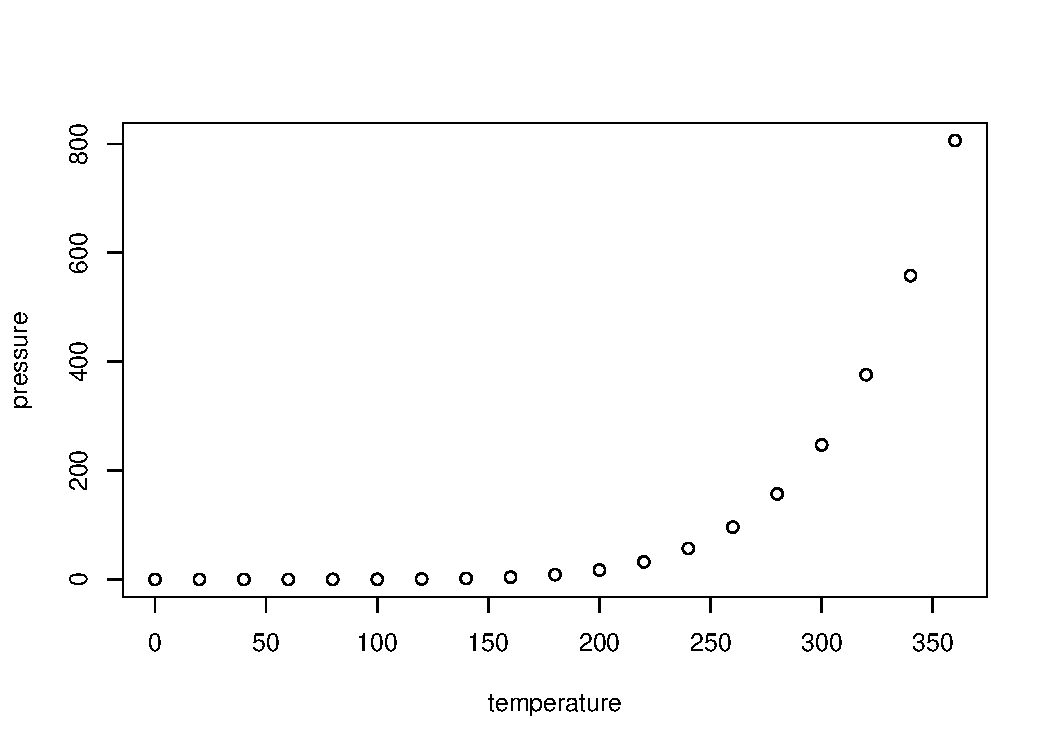
\includegraphics{Guideline-Book_files/figure-latex/pressure-1.pdf}

Note that the \texttt{echo\ =\ FALSE} parameter was added to the code
chunk to prevent printing of the R code that generated the plot.

\newpage

\section{R PROGRAMMING}\label{r-programming}

\textbf{R} is a programming language and software environment for
statistical computing and graphics. It is widely used among
statisticians and data miners for developing statistical software and
data analysis. Use of a software is desirable and moreover an essential
part of any analysis. It supports many free packages which helps the
data scientist and analyst.It is a \textbf{free software}.

R Programming is Developed by \textbf{Ross Ihaka and Robert Gentleman}
in 1993. It is dialect of \textbf{S language.} which was developed at
Bell Laboratories by \textbf{John Chambers} and colleagues.

\textbf{what is R ?}

\begin{itemize}
\item
  R is an environment for data manipulation, statistical computing,
  graphics display and data analysis.
\item
  Effective data handling and storage of outputs is possible.
\item
  Simple as well as complicated calculations are possible.
\item
  Simulations are possible.
\item
  Graphical display on‐screen and hard copy are possible.
\item
  Programming language is effective which includes all possibilities
  just like any other good programming language.
\item
  R has a statistical computing environment.
\item
  It has a computer language which is convenient to use for statistical
  and graphical applications.
\end{itemize}

\ul{\textbf{Installing R}}

\begin{itemize}
\tightlist
\item
  \textbf{Download the R software} from the Comprehensive R Archive
  Network (CRAN)
  website:\href{https://cran.r-project.org/}{\textbf{https://cran.r-project.org/}}
\end{itemize}

\ul{\textbf{Working with R}}

\begin{itemize}
\item
  Use commandline to type and execute the commands
\item
  Some free software like \textbf{R Studio, Tinn R} etc. are also
  available to work with R software. It is an interface between R and us
  .
\item
  Such software are more useful for beginners.
\item
  It makes coding and execution of programmes easier
\item
  \textbf{RStudio} is available at
  \href{https://www.rstudio.com/}{\textbf{https://www.rstudio.com/}}
\item
  \textbf{Tinn R} is available at
  \href{https://sourceforge.net/projects/tinn‐r/}{\textbf{https://sourceforge.net/projects/tinn‐r/}}
\end{itemize}

\ul{\textbf{Features of R Programming :}}

\begin{itemize}
\item
  Free to Run and Use
\item
  Free to Study
\item
  Free to Share
\item
  Free to update
\end{itemize}

\subsection{R Operators}\label{r-operators}

There are several types of operators in R programming. They are :

\begin{itemize}
\item
  Assignment Operators
\item
  Arithmetic Operators
\item
  Relational Operators
\item
  Logical Operators
\item
  Miscellaneous Operators
\end{itemize}

\ul{\textbf{Assignment Operators}}

\begin{Shaded}
\begin{Highlighting}[]
\OtherTok{\textless{}{-}}  \SpecialCharTok{{-}}\OtherTok{{-}\textgreater{}}\NormalTok{ Leftward Assignment}
\OtherTok{{-}\textgreater{}}  \SpecialCharTok{{-}}\OtherTok{{-}\textgreater{}}\NormalTok{ Rightward Assignment}
\OtherTok{{-}\textgreater{}\textgreater{}} \SpecialCharTok{{-}}\OtherTok{{-}\textgreater{}}\NormalTok{ Rightward Assignment}
\OtherTok{=}   \SpecialCharTok{{-}}\OtherTok{{-}\textgreater{}}\NormalTok{ Assignment}
\end{Highlighting}
\end{Shaded}

Example for Assignment Operators:

\begin{enumerate}
\def\labelenumi{\arabic{enumi}.}
\tightlist
\item
  \textbf{Leftward Assignment:}
\end{enumerate}

\begin{Shaded}
\begin{Highlighting}[]
\NormalTok{a }\OtherTok{\textless{}{-}} \DecValTok{10}
\NormalTok{a1 }\OtherTok{\textless{}\textless{}{-}} \DecValTok{100}
\FunctionTok{print}\NormalTok{(}\FunctionTok{c}\NormalTok{(a,a1))}
\end{Highlighting}
\end{Shaded}

\begin{verbatim}
## [1]  10 100
\end{verbatim}

\begin{enumerate}
\def\labelenumi{\arabic{enumi}.}
\setcounter{enumi}{1}
\tightlist
\item
  \textbf{Rightward Assignment:}
\end{enumerate}

\begin{Shaded}
\begin{Highlighting}[]
\DecValTok{11} \OtherTok{{-}\textgreater{}}\NormalTok{ b}
\DecValTok{111} \OtherTok{{-}\textgreater{}\textgreater{}}\NormalTok{ b1}
\FunctionTok{print}\NormalTok{(}\FunctionTok{c}\NormalTok{(b,b1))}
\end{Highlighting}
\end{Shaded}

\begin{verbatim}
## [1]  11 111
\end{verbatim}

\begin{enumerate}
\def\labelenumi{\arabic{enumi}.}
\setcounter{enumi}{2}
\tightlist
\item
  \textbf{Equal Assignment:}
\end{enumerate}

\begin{Shaded}
\begin{Highlighting}[]
\NormalTok{c }\OtherTok{=} \DecValTok{12}
\FunctionTok{print}\NormalTok{(c)}
\end{Highlighting}
\end{Shaded}

\begin{verbatim}
## [1] 12
\end{verbatim}

\ul{\textbf{Arithmetic Operators}}

\begin{Shaded}
\begin{Highlighting}[]
\SpecialCharTok{+} \OtherTok{{-}\textgreater{}}\NormalTok{ Addition}
\SpecialCharTok{{-}} \OtherTok{{-}\textgreater{}}\NormalTok{ Subtraction }
\SpecialCharTok{*} \OtherTok{{-}\textgreater{}}\NormalTok{ Multiplication}
\SpecialCharTok{/} \OtherTok{{-}\textgreater{}}\NormalTok{ Division}
\SpecialCharTok{**}\NormalTok{ or }\SpecialCharTok{\^{}} \OtherTok{{-}\textgreater{}}\NormalTok{ For power or Exponential}
\SpecialCharTok{\%\%} \OtherTok{{-}\textgreater{}}\NormalTok{ Modulus}
\SpecialCharTok{\%/\%} \OtherTok{{-}\textgreater{}}\NormalTok{ Integer Division}
\end{Highlighting}
\end{Shaded}

Example for Arithmetic Operators:

\begin{Shaded}
\begin{Highlighting}[]
\DecValTok{1}\SpecialCharTok{+}\DecValTok{1} \CommentTok{\# Addition}
\end{Highlighting}
\end{Shaded}

\begin{verbatim}
## [1] 2
\end{verbatim}

\begin{Shaded}
\begin{Highlighting}[]
\DecValTok{2{-}1} \CommentTok{\# Subtraction}
\end{Highlighting}
\end{Shaded}

\begin{verbatim}
## [1] 1
\end{verbatim}

\begin{Shaded}
\begin{Highlighting}[]
\DecValTok{3}\SpecialCharTok{*}\DecValTok{2} \CommentTok{\# Multiplication}
\end{Highlighting}
\end{Shaded}

\begin{verbatim}
## [1] 6
\end{verbatim}

\begin{Shaded}
\begin{Highlighting}[]
\DecValTok{4}\SpecialCharTok{/}\DecValTok{2} \CommentTok{\# Division}
\end{Highlighting}
\end{Shaded}

\begin{verbatim}
## [1] 2
\end{verbatim}

\begin{Shaded}
\begin{Highlighting}[]
\DecValTok{5}\SpecialCharTok{\^{}}\DecValTok{2} \CommentTok{\# Exponential}
\end{Highlighting}
\end{Shaded}

\begin{verbatim}
## [1] 25
\end{verbatim}

\begin{Shaded}
\begin{Highlighting}[]
\DecValTok{5}\SpecialCharTok{**}\DecValTok{2} \CommentTok{\# Exponential}
\end{Highlighting}
\end{Shaded}

\begin{verbatim}
## [1] 25
\end{verbatim}

\begin{Shaded}
\begin{Highlighting}[]
\DecValTok{5}\SpecialCharTok{\%\%}\DecValTok{2} \CommentTok{\# Modulus (the remainder will be the result)}
\end{Highlighting}
\end{Shaded}

\begin{verbatim}
## [1] 1
\end{verbatim}

\begin{Shaded}
\begin{Highlighting}[]
\DecValTok{5}\SpecialCharTok{\%/\%}\DecValTok{2} \CommentTok{\# Integer Division}
\end{Highlighting}
\end{Shaded}

\begin{verbatim}
## [1] 2
\end{verbatim}

\ul{\textbf{Relational Operators}}

The Result of Relational Operators is always a \textbf{Boolean Value}
(True or False)

\begin{Shaded}
\begin{Highlighting}[]
\SpecialCharTok{\textless{}}  \SpecialCharTok{{-}}\OtherTok{{-}\textgreater{}}\NormalTok{ Less than }
\SpecialCharTok{\textgreater{}}  \SpecialCharTok{{-}}\OtherTok{{-}\textgreater{}}\NormalTok{ Greater than}
\SpecialCharTok{\textless{}=} \SpecialCharTok{{-}}\OtherTok{{-}\textgreater{}}\NormalTok{ Less than or equal to}
\SpecialCharTok{\textgreater{}=} \SpecialCharTok{{-}}\OtherTok{{-}\textgreater{}}\NormalTok{ Greater than or equal to}
\SpecialCharTok{==} \SpecialCharTok{{-}}\OtherTok{{-}\textgreater{}}\NormalTok{ Equal to }
\SpecialCharTok{!=} \SpecialCharTok{{-}}\OtherTok{{-}\textgreater{}}\NormalTok{ Not Equal to }
\end{Highlighting}
\end{Shaded}

Example for Relational Operators:

\begin{Shaded}
\begin{Highlighting}[]
\NormalTok{a }\OtherTok{=} \DecValTok{10}
\NormalTok{b}\OtherTok{=}\DecValTok{20}
\FunctionTok{print}\NormalTok{(}\FunctionTok{c}\NormalTok{(a,b))}
\end{Highlighting}
\end{Shaded}

\begin{verbatim}
## [1] 10 20
\end{verbatim}

\begin{Shaded}
\begin{Highlighting}[]
\NormalTok{a}\SpecialCharTok{\textless{}}\NormalTok{b}
\end{Highlighting}
\end{Shaded}

\begin{verbatim}
## [1] TRUE
\end{verbatim}

\begin{Shaded}
\begin{Highlighting}[]
\NormalTok{a}\SpecialCharTok{\textgreater{}}\NormalTok{b}
\end{Highlighting}
\end{Shaded}

\begin{verbatim}
## [1] FALSE
\end{verbatim}

\begin{Shaded}
\begin{Highlighting}[]
\NormalTok{a}\SpecialCharTok{\textless{}=}\NormalTok{b}
\end{Highlighting}
\end{Shaded}

\begin{verbatim}
## [1] TRUE
\end{verbatim}

\begin{Shaded}
\begin{Highlighting}[]
\NormalTok{a}\SpecialCharTok{\textgreater{}=}\NormalTok{b}
\end{Highlighting}
\end{Shaded}

\begin{verbatim}
## [1] FALSE
\end{verbatim}

\begin{Shaded}
\begin{Highlighting}[]
\NormalTok{a}\SpecialCharTok{==}\NormalTok{b}
\end{Highlighting}
\end{Shaded}

\begin{verbatim}
## [1] FALSE
\end{verbatim}

\begin{Shaded}
\begin{Highlighting}[]
\NormalTok{a}\SpecialCharTok{!=}\NormalTok{b}
\end{Highlighting}
\end{Shaded}

\begin{verbatim}
## [1] TRUE
\end{verbatim}

\newpage

\ul{\textbf{Logical Operators:}}

Logical operators are used to combine conditional statements. it returns
a boolean value (True or False)

\begin{Shaded}
\begin{Highlighting}[]
\SpecialCharTok{\&} \OtherTok{{-}\textgreater{}}\NormalTok{ AND}
\SpecialCharTok{\&\&} \OtherTok{{-}\textgreater{}}\NormalTok{ Logical And}
\SpecialCharTok{|} \OtherTok{{-}\textgreater{}}\NormalTok{OR}
\SpecialCharTok{||} \OtherTok{{-}\textgreater{}}\NormalTok{ Logical OR}
\SpecialCharTok{!} \OtherTok{{-}\textgreater{}}\NormalTok{ NOT}
\end{Highlighting}
\end{Shaded}

Example for Logical Operators:

\begin{Shaded}
\begin{Highlighting}[]
\NormalTok{a }\OtherTok{=} \DecValTok{10}
\NormalTok{b}\OtherTok{=}\DecValTok{20}
\FunctionTok{print}\NormalTok{(}\FunctionTok{c}\NormalTok{(a,b))}
\end{Highlighting}
\end{Shaded}

\begin{verbatim}
## [1] 10 20
\end{verbatim}

\begin{Shaded}
\begin{Highlighting}[]
\CommentTok{\# And Operator}
\CommentTok{\# The Statement both should be true to get the result as true}
\CommentTok{\# Any one of the statement is false then the result will be \#false}
\NormalTok{a}\SpecialCharTok{==}\DecValTok{10} \SpecialCharTok{\&}\NormalTok{ b}\SpecialCharTok{==}\DecValTok{20}
\end{Highlighting}
\end{Shaded}

\begin{verbatim}
## [1] TRUE
\end{verbatim}

\begin{Shaded}
\begin{Highlighting}[]
\NormalTok{a}\SpecialCharTok{==}\DecValTok{10} \SpecialCharTok{\&}\NormalTok{ b}\SpecialCharTok{==}\DecValTok{30}
\end{Highlighting}
\end{Shaded}

\begin{verbatim}
## [1] FALSE
\end{verbatim}

\begin{Shaded}
\begin{Highlighting}[]
\CommentTok{\# OR Operator}
\CommentTok{\# The Statement any one should be true to get the result as \#true}
\CommentTok{\# Both the statement is false then the result will be false}
\NormalTok{a}\SpecialCharTok{==}\DecValTok{10} \SpecialCharTok{|}\NormalTok{ b}\SpecialCharTok{==}\DecValTok{30}
\end{Highlighting}
\end{Shaded}

\begin{verbatim}
## [1] TRUE
\end{verbatim}

\begin{Shaded}
\begin{Highlighting}[]
\NormalTok{a}\SpecialCharTok{==}\DecValTok{20} \SpecialCharTok{|}\NormalTok{ b}\SpecialCharTok{==}\DecValTok{30}
\end{Highlighting}
\end{Shaded}

\begin{verbatim}
## [1] FALSE
\end{verbatim}

\begin{Shaded}
\begin{Highlighting}[]
\CommentTok{\# NOT Operator}
\CommentTok{\# The Statement should be false to get the result as true}
\CommentTok{\# The Statement should be true to get the result as false}
\NormalTok{a}\SpecialCharTok{!=}\DecValTok{10}
\end{Highlighting}
\end{Shaded}

\begin{verbatim}
## [1] FALSE
\end{verbatim}

\begin{Shaded}
\begin{Highlighting}[]
\NormalTok{a}\SpecialCharTok{!=}\DecValTok{20}
\end{Highlighting}
\end{Shaded}

\begin{verbatim}
## [1] TRUE
\end{verbatim}

\ul{\textbf{Miscellaneous Operators}}

In R, miscellaneous operators are special operators that don't fall into
typical arithmetic, logical, or relational categories. Some important
ones include:

\begin{Shaded}
\begin{Highlighting}[]
\NormalTok{ x }\OtherTok{\textless{}{-}} \FunctionTok{c}\NormalTok{(}\DecValTok{1}\NormalTok{, }\DecValTok{2}\NormalTok{, }\DecValTok{3}\NormalTok{, }\DecValTok{4}\NormalTok{, }\DecValTok{5}\NormalTok{)}
\NormalTok{y }\OtherTok{\textless{}{-}} \FunctionTok{c}\NormalTok{(}\DecValTok{2}\NormalTok{, }\DecValTok{4}\NormalTok{, }\DecValTok{6}\NormalTok{)}
\NormalTok{x }\SpecialCharTok{\%in\%}\NormalTok{ y}
\end{Highlighting}
\end{Shaded}

\begin{verbatim}
## [1] FALSE  TRUE FALSE  TRUE FALSE
\end{verbatim}

\begin{Shaded}
\begin{Highlighting}[]
\DecValTok{1}\SpecialCharTok{:}\DecValTok{5} \CommentTok{\# Sequence from 1 to 5}
\end{Highlighting}
\end{Shaded}

\begin{verbatim}
## [1] 1 2 3 4 5
\end{verbatim}

\begin{Shaded}
\begin{Highlighting}[]
\FunctionTok{seq}\NormalTok{(}\DecValTok{1}\NormalTok{,}\DecValTok{10}\NormalTok{,}\AttributeTok{by=}\DecValTok{2}\NormalTok{) }\CommentTok{\# With Difference of 2}
\end{Highlighting}
\end{Shaded}

\begin{verbatim}
## [1] 1 3 5 7 9
\end{verbatim}

\begin{Shaded}
\begin{Highlighting}[]
\FunctionTok{seq}\NormalTok{(}\DecValTok{1}\NormalTok{,}\DecValTok{10}\NormalTok{,}\AttributeTok{length=}\DecValTok{3}\NormalTok{) }\CommentTok{\# the output should be 3 numbers between 1 to 10  }
\end{Highlighting}
\end{Shaded}

\begin{verbatim}
## [1]  1.0  5.5 10.0
\end{verbatim}

\begin{Shaded}
\begin{Highlighting}[]
 \CommentTok{\# $}
\NormalTok{df }\OtherTok{\textless{}{-}} \FunctionTok{data.frame}\NormalTok{(}\AttributeTok{Name =} \FunctionTok{c}\NormalTok{(}\StringTok{"A"}\NormalTok{, }\StringTok{"B"}\NormalTok{), }\AttributeTok{Age =} \FunctionTok{c}\NormalTok{(}\DecValTok{25}\NormalTok{, }\DecValTok{30}\NormalTok{))}
\NormalTok{df}\SpecialCharTok{$}\NormalTok{Name}
\end{Highlighting}
\end{Shaded}

\begin{verbatim}
## [1] "A" "B"
\end{verbatim}

Data Types in R In R, data types are classified into two type.

\begin{itemize}
\item
  Object
\item
  Attributes
\end{itemize}

There are 5 basic data types in Object:

\begin{enumerate}
\def\labelenumi{\arabic{enumi}.}
\item
  Numeric
\item
  Integer
\item
  Complex
\item
  Logical
\item
  Character
\end{enumerate}

There are 6 basic data types in Attributes:

\begin{enumerate}
\def\labelenumi{\arabic{enumi}.}
\item
  Vectors
\item
  Factors
\item
  Lists
\item
  Arrays / Matrics
\item
  Data Frames
\item
  Class
\end{enumerate}

We can use \texttt{Typeof()} function to check the data type of the
object. The Result for typeof function will be

\begin{Shaded}
\begin{Highlighting}[]
\NormalTok{integer }\OtherTok{{-}\textgreater{}}\NormalTok{ integer}
\NormalTok{character }\OtherTok{{-}\textgreater{}}\NormalTok{ Character}
\NormalTok{logical }\OtherTok{{-}\textgreater{}}\NormalTok{ Logical}
\NormalTok{numeric }\OtherTok{{-}\textgreater{}}\NormalTok{ Double}
\NormalTok{complex }\OtherTok{{-}\textgreater{}}\NormalTok{ Complex}
\NormalTok{Factor }\OtherTok{{-}\textgreater{}}\NormalTok{ Factor}
\end{Highlighting}
\end{Shaded}

\begin{Shaded}
\begin{Highlighting}[]
 \CommentTok{\# $}
\NormalTok{a}\OtherTok{=}\DecValTok{10}
\FunctionTok{typeof}\NormalTok{(a)}
\end{Highlighting}
\end{Shaded}

\begin{verbatim}
## [1] "double"
\end{verbatim}

\newpage

we can use as. , is. functions to check and change the data type

\begin{Shaded}
\begin{Highlighting}[]
\CommentTok{\# is function is used to check the data type}
\CommentTok{\# if the data type is correct then it will return as true otherwise False}
\FunctionTok{is.numeric}\NormalTok{()}
\FunctionTok{is.integer}\NormalTok{()}
\FunctionTok{is.character}\NormalTok{()}
\FunctionTok{is.logical}\NormalTok{()}
\FunctionTok{is.complex}\NormalTok{()}
\FunctionTok{is.factor}\NormalTok{()}
\FunctionTok{is.vector}\NormalTok{()}
\FunctionTok{is.list}\NormalTok{()}
\FunctionTok{is.matrix}\NormalTok{()}
\FunctionTok{is.data.frame}\NormalTok{()}
\FunctionTok{is.array}\NormalTok{()}
\end{Highlighting}
\end{Shaded}

Like this there are more functions available in R to check the data type
of the object.

\begin{Shaded}
\begin{Highlighting}[]
\CommentTok{\# as function is used to change the data type}
\FunctionTok{as.numeric}\NormalTok{() }\CommentTok{\# To change the data type to numeric}
\FunctionTok{as.integer}\NormalTok{() }\CommentTok{\# To change the data type to integer}
\FunctionTok{as.character}\NormalTok{() }\CommentTok{\# To change the data type to character}
\FunctionTok{as.logical}\NormalTok{() }\CommentTok{\# To change the data type to logical}
\FunctionTok{as.matrix}\NormalTok{() }\CommentTok{\# To change the data type to matrix}
\FunctionTok{as.data.frame}\NormalTok{() }\CommentTok{\# To change the data type to data frame}
\FunctionTok{as.vector}\NormalTok{() }\CommentTok{\# To change the data type to vector}
\FunctionTok{as.factor}\NormalTok{() }\CommentTok{\# To change the data type to factor}
\end{Highlighting}
\end{Shaded}

\ul{\textbf{Using R as a Calculator}}

We can use R as a basic calculator to perform arithmetic operations. For
example, we can add, subtract, multiply, and divide numbers using R.

\textbf{Multiple operators (BODMAS):}

\begin{Shaded}
\begin{Highlighting}[]
 \DecValTok{6}\SpecialCharTok{+}\DecValTok{5{-}4}\SpecialCharTok{*}\DecValTok{3}\SpecialCharTok{+}\DecValTok{2}\SpecialCharTok{/}\DecValTok{4}
\end{Highlighting}
\end{Shaded}

\begin{verbatim}
## [1] -0.5
\end{verbatim}

\textbf{Concatenate:}

Still now we have seen that using single value for the operation. But we
can also use multiple values for the operation. by using concatenate.

\begin{Shaded}
\begin{Highlighting}[]
\NormalTok{x}\OtherTok{=}\FunctionTok{c}\NormalTok{(}\DecValTok{1}\NormalTok{,}\DecValTok{2}\NormalTok{,}\DecValTok{3}\NormalTok{,}\DecValTok{4}\NormalTok{.......)}
\NormalTok{allow us to use multiple values }\ControlFlowTok{for}\NormalTok{ the operation}
\end{Highlighting}
\end{Shaded}

While using concatenate we can use multiple values but in a same data
type

\begin{Shaded}
\begin{Highlighting}[]
\NormalTok{ x}\OtherTok{=}\FunctionTok{c}\NormalTok{(}\DecValTok{1}\NormalTok{,}\DecValTok{2}\NormalTok{,}\DecValTok{3}\NormalTok{,}\DecValTok{4}\NormalTok{) }\CommentTok{\# Multiple values}
\FunctionTok{print}\NormalTok{(x)}
\end{Highlighting}
\end{Shaded}

\begin{verbatim}
## [1] 1 2 3 4
\end{verbatim}

\newpage

\section{Git / GitHub}\label{git-github}

\textbf{Git} Terminology Features and Advantages of Git TerminologyGit
is a free, open-source \textbf{version control system (VCS)} that helps
manage source code and its development history. It's the most widely
used VCS in the world

\textbf{GitHub} is a website that helps developers store, manage, and
collaborate on software projects.It's a social network for programmers
that encourages collaboration and sharing of code . Github is an online
platform that allows you to store remote repositories of your projects
(Interactable)

\subsection{SOURCE CONTROL / VERSION
CONTROL}\label{source-control-version-control}

\begin{itemize}
\tightlist
\item
  Some System used for tracking your file progress over time .
\item
  It is usually saved in a series of snapshots and branches, which you
  can move back and forth between.
\item
  Prevent against data loss / damage by Creating backup copies of your
  work.
\end{itemize}

Linux is the major / huge project in github Git is a Source Control
Software . It was created by the same person who created Linux
\textbf{Linus Torvalds}

\subsection{Command Prompt}\label{command-prompt}

Before using git/github we need to have a basic idea about command
prompt . Command prompt is a command line interpreter application
available in most Windows operating systems. It's used to execute
entered commands. Most of those commands automate tasks via scripts and
batch files, perform advanced administrative functions, and troubleshoot
or solve certain kinds of Windows issues.

Some of the basic commands prompt codes are :

\begin{Shaded}
\begin{Highlighting}[]
\NormalTok{E}\SpecialCharTok{:} \OtherTok{{-}\textgreater{}}\NormalTok{ To change the drive to E}
\NormalTok{cd }\OtherTok{{-}\textgreater{}}\NormalTok{ To change the directory}

\CommentTok{\# some time we have space in the directory name so we need to use double quotes}
\NormalTok{cd }\StringTok{"C:\textbackslash{}Users\textbackslash{}Deepaneesh R V\textbackslash{}Documents"} \OtherTok{{-}\textgreater{}}\NormalTok{ To change the directory to Documents}
\NormalTok{cd.. }\OtherTok{{-}\textgreater{}}\NormalTok{ To go back to the previous directory}
\NormalTok{cd}\SpecialCharTok{/} \OtherTok{{-}\textgreater{}}\NormalTok{ To go to the root }\FunctionTok{directory}\NormalTok{(Home)}
\NormalTok{cd}\SpecialCharTok{/}\NormalTok{mnt}\SpecialCharTok{/}\NormalTok{E }\OtherTok{{-}\textgreater{}}\NormalTok{ To change the directory to E drive }
\NormalTok{dir }\OtherTok{{-}\textgreater{}}\NormalTok{To list the files }\ControlFlowTok{in}\NormalTok{ the directory}
\end{Highlighting}
\end{Shaded}

\textbf{Folder Creation} Their is a command to create a new
directory(Folder) and to remove a directory( Folder)

like:

\begin{Shaded}
\begin{Highlighting}[]
\NormalTok{mkdir }\OtherTok{{-}\textgreater{}}\NormalTok{ To create a new }\FunctionTok{directory}\NormalTok{(Folder)}
\NormalTok{rmdir }\OtherTok{{-}\textgreater{}}\NormalTok{ To remove a }\FunctionTok{directory}\NormalTok{( Folder)}
\end{Highlighting}
\end{Shaded}

\textbf{File Creation} Their is a command to create a new file and to
remove a file

like:

\begin{Shaded}
\begin{Highlighting}[]
\NormalTok{echo }\StringTok{"Hello"} \SpecialCharTok{\textgreater{}}\NormalTok{ hello.txt }\SpecialCharTok{|{-}}\OtherTok{{-}\textgreater{}}\NormalTok{ To create a new file}
\NormalTok{type null }\SpecialCharTok{\textgreater{}}\NormalTok{ hello.txt }\SpecialCharTok{|{-}}\OtherTok{{-}\textgreater{}}\NormalTok{ To create a new file}
\NormalTok{copy con hello.txt }\SpecialCharTok{|{-}}\OtherTok{{-}\textgreater{}}\NormalTok{ To create a new file}
\NormalTok{del hello.txt }\SpecialCharTok{|{-}}\OtherTok{{-}\textgreater{}}\NormalTok{ To remove a file}
\NormalTok{del . }\SpecialCharTok{|{-}}\OtherTok{{-}\textgreater{}}\NormalTok{ To remove all the files }\ControlFlowTok{in}\NormalTok{ the directory}
\end{Highlighting}
\end{Shaded}

\textbf{Repository} A repository is a storage space where your project
lives. It can be local to a folder on your computer or it can be a
storage space on GitHub or another online platform.

\begin{Shaded}
\begin{Highlighting}[]
\NormalTok{local repository }\OtherTok{{-}\textgreater{}}\NormalTok{ Repository }\ControlFlowTok{in}\NormalTok{ your computer}
\NormalTok{Remote repository }\OtherTok{{-}\textgreater{}}\NormalTok{ Repository }\ControlFlowTok{in}\NormalTok{ the }\FunctionTok{cloud}\NormalTok{ (Github)}
\end{Highlighting}
\end{Shaded}

Respositories are the timelines of the entire project including the
previous changes

\textbf{Git Commands} Before using git we need to install git in our
system. then you need to configure the git with your username and email
id. Code for Configuring the git (Only for the first time) like
Registering the git with your username and email id

\begin{Shaded}
\begin{Highlighting}[]
\NormalTok{git config }\SpecialCharTok{{-}{-}}\NormalTok{global user.name }\StringTok{"Username"}
\NormalTok{git config }\SpecialCharTok{{-}{-}}\NormalTok{global user.email }\StringTok{"Email id"}
\end{Highlighting}
\end{Shaded}

\textbf{Flow Chart of Github}

\begin{Shaded}
\begin{Highlighting}[]
\NormalTok{Untracked }\OtherTok{{-}\textgreater{}}\NormalTok{ Staged }\OtherTok{{-}\textgreater{}}\NormalTok{ Committed }\OtherTok{{-}\textgreater{}}\NormalTok{ Uploading}
          \SpecialCharTok{|}         \ErrorTok{|}            \ErrorTok{|}
\NormalTok{        (add)    (Commit)       (Push)}
\end{Highlighting}
\end{Shaded}

This is the flow chart of github

\textbf{Git basic Command}

\begin{Shaded}
\begin{Highlighting}[]
\NormalTok{git init                     }\SpecialCharTok{|{-}{-}}\OtherTok{{-}\textgreater{}}\NormalTok{ initializing the git}
\NormalTok{git add .                    }\SpecialCharTok{|{-}{-}}\OtherTok{{-}\textgreater{}}\NormalTok{ add everything}
\NormalTok{git commit }\SpecialCharTok{{-}}\NormalTok{m }\StringTok{"first commit"} \SpecialCharTok{|{-}{-}}\OtherTok{{-}\textgreater{}}\NormalTok{ commit }
\NormalTok{git remote add origin git}\SpecialCharTok{@}\NormalTok{github.com}\SpecialCharTok{:}\NormalTok{username}\SpecialCharTok{/}\ErrorTok{\textless{}}\NormalTok{reponame}\SpecialCharTok{\textgreater{}}\NormalTok{.git   }\SpecialCharTok{|{-}{-}}\OtherTok{{-}\textgreater{}}\NormalTok{choosing the git website }\ControlFlowTok{for}\NormalTok{ loading}
\NormalTok{git push }\SpecialCharTok{{-}}\NormalTok{u origin master    }\SpecialCharTok{|{-}{-}}\OtherTok{{-}\textgreater{}}\NormalTok{ pushing the changes to github }
\end{Highlighting}
\end{Shaded}


\end{document}
